\documentclass[a4paper,fleqn]{cas-sc}

\usepackage[numbers]{natbib}
\usepackage{amsmath,amssymb,amsfonts}
\usepackage{algorithm}
\usepackage{algorithmic}
\usepackage{graphicx}
\usepackage{textcomp}
\usepackage{xcolor}
\usepackage{booktabs}
\usepackage{multirow}
\usepackage{subcaption}
\usepackage{fancyhdr}
\usepackage{url}
\usepackage{microtype}
\usepackage{hyperref}
\usepackage{lastpage}
\usepackage{helvet}
\usepackage[margin=1.4cm]{geometry}
\usepackage[utf8]{inputenc}
\usepackage[table]{xcolor}
\usepackage{tabularx}
\usepackage{array}

\begin{document}

\pagestyle{plain}
\fancyhf{}
\fancyfoot[C]{\thepage\ / \pageref{LastPage}}

\let\WriteBookmarks\relax
\def\floatpagepagefraction{1}
\def\textpagefraction{.001}

\renewcommand{\familydefault}{\sfdefault}
\renewcommand{\arraystretch}{1.4}
\setlength{\parindent}{0pt}
\setlength{\tabcolsep}{4pt}

\definecolor{TitleBlue}{RGB}{53,56,108}
\definecolor{RowGray}{RGB}{240,240,240}
\definecolor{TextBlue}{RGB}{31,63,139}
\definecolor{BorderGray}{RGB}{195,195,195}

\hypersetup{
    colorlinks=true,
    urlcolor=TextBlue,
    linkcolor=TextBlue
}

\arrayrulecolor{BorderGray}

\thispagestyle{empty}

\begin{center}
    \vspace*{0.8cm}

    {\color{TitleBlue}\fontsize{23}{27}\selectfont
    \textbf{Discrete Optimization}\par}

    \vspace{0.12cm}

    {\color{TitleBlue}\fontsize{17}{20}\selectfont
    \textbf{SAT Solving for the N-Queens Problem}\par}

    {\color{TitleBlue}\fontsize{13}{16}\selectfont
    -- Project Report --\par}

    \vspace{0.55cm}
\end{center}

\noindent
\begin{tabularx}{\textwidth}{
    |>{\raggedright\arraybackslash
    \color{TitleBlue}\bfseries}p{0.32\textwidth}
    |>{\raggedright\arraybackslash
    \color{TextBlue}}X|
}
\hline

\rowcolor{RowGray}
Project ID: & NQ-SAT-01 \\
\hline

Project Type: & Large Assignment \\
\hline

Keywords: &
N-Queens Problem, SAT Solver, Boolean Variables,
Logical Constraints, Discrete Optimization. \\
\hline

Author: & Nguyen Viet Nhuong \\
\hline

Problem Statement: &
Place $N$ queens on an $N \times N$ chessboard
so that no two queens attack each other. \\
\hline

Methodology: &
Encode the constraints as a Boolean formula and use
a SAT solver to find a valid configuration. \\
\hline

Abstract: &
This project applies SAT solving to the N-Queens
problem by constructing Boolean variables and logical
constraints, then evaluating the solver's ability
to find valid solutions. \\
\hline

GitHub Repository: &
\href{https://github.com/YwliF/BTL_01}
{\textcolor{TextBlue}{github.com/YwliF/BTL\_01}} \\
\hline

\end{tabularx}

% The custom cover is unnumbered; restart numbering on the next page.
\clearpage
\pagenumbering{arabic}
\setcounter{page}{1}

\begin{keywords}
$N$-Queens \sep Boolean Satisfiability (SAT) \sep Cardinality encodings \sep Mixed-Integer Programming \sep Constraint Programming \sep PySAT \sep Gurobi \sep CP-SAT \sep Reproducibility
\end{keywords}

\maketitle

\pagestyle{fancy}
\fancyhf{}
\fancyfoot[C]{\thepage\ / \pageref{LastPage}}
\thispagestyle{fancy}

\section{Introduction}
\label{sec:intro}

The $N$-Queens problem is a classical constraint satisfaction benchmark: place $N$ chess queens on an $N\times N$ board so that no two queens attack one another~\cite{bell2009survey,sosic1994local}.
For $N=1$ the problem is trivial; for $N\in\{2,3\}$ it is unsatisfiable; and for every $N\ge 4$ a solution exists~\cite{bell2009survey}.
The decision version is therefore not hard in the existence sense.
The engineering problem, however, is still substantial.
Encodings grow with $N$, SAT engines expose very different restart and clause-management policies, MIP solvers are sensitive to licence size caps, and implementation errors are easy to hide unless solutions are checked independently of the constraint model.

Modern exact solving provides three mature routes to the same specification~\cite{biere2021handbook}:
\begin{itemize}
    \item \textbf{SAT.} Conflict-driven clause learning (CDCL) solvers decide CNF formulas.
    Cardinality constraints must be encoded explicitly, and the choice of encoding changes both formula size and unit-propagation strength~\cite{sinz2005towards,ignatiev2018pysat,audemard2018glucose}.
    \item \textbf{MIP.} Zero--one linear models are handled by LP relaxation, cutting planes, and branch-and-bound in Gurobi and CPLEX~\cite{gurobi2024,cplex2024}.
    \item \textbf{CP.} Global constraints, especially R{\'e}gin's \texttt{AllDifferent} propagator~\cite{regin1994filtering}, combined with clause learning in CP-SAT~\cite{perron2024ortools}, operate directly on integer permutation variables.
\end{itemize}

This report treats $N$-Queens as a controlled laboratory for comparing those routes on one codebase, one machine, and one measurement protocol.
The scientific questions are:
\begin{enumerate}
    \item How do five standard At-Most-One (AMO) encodings change CNF size, auxiliary variables, and SAT search time?
    \item How do five CDCL engines behave on an identical Sequential Counter formula?
    \item How do SAT, Gurobi MIP, CPLEX, and CP-SAT compare under the available academic/community licenses and a 60-second cutoff?
    \item Which paradigm remains practical as $N$ grows from recreational boards to $N=500$?
\end{enumerate}

The remainder of the report is organised as follows.
Section~\ref{sec:design} states how the report structure was designed to match the instructor's requirement and lists concrete contributions.
Section~\ref{sec:background} reviews cardinality encodings and exact solvers.
Section~\ref{sec:problem} gives the mathematical model.
Sections~\ref{sec:sat} and~\ref{sec:mipcp} describe SAT, MIP, and CP formulations.
Section~\ref{sec:impl} documents the software architecture and correctness pipeline.
Section~\ref{sec:setup} specifies the experimental protocol.
Section~\ref{sec:results} reports Experiments A--E.
Section~\ref{sec:discussion} interprets the measurements.
Section~\ref{sec:threats} discusses limitations.
Section~\ref{sec:data} is the Data Availability section requested by the instructor, with the public GitHub URL.
Section~\ref{sec:conclusion} concludes.

\section{Report design and contributions}
\label{sec:design}

\subsection{Why the structure is not a copied outline}
The sample manuscript provided for BTL~1 and BTL~2 is an Elsevier CAS paper on exact SAT solving.
Students are encouraged to design their own structure and content so that the report exhibits what was actually implemented and measured.
Copying the section titles of a graph-layout paper would hide the work of this assignment.
The present document therefore keeps the CAS front matter (title, abstract, highlights, keywords, numbered citations) but organises the body around artefacts that exist in the repository:
\begin{itemize}
    \item a reusable Python package (\texttt{src/nqueens/}) with encodings, solvers, validation, and experiment orchestration;
    \item an automated test suite and a cross-solver correctness script;
    \item five benchmark campaigns (Experiments A--E) stored as CSV;
    \item publication figures generated from those CSV files;
    \item this Elsevier CAS single-column manuscript~\cite{casbundle}.
\end{itemize}

\subsection{Contributions}
\begin{enumerate}
    \item A verified implementation of Pairwise, Sequential Counter~\cite{sinz2005towards}, Commander~\cite{klieber2007commander}, Product~\cite{chen2010new}, and Binary~\cite{frisch2005symmetry} encodings for $N$-Queens.
    \item Bindings to Glucose~4, CaDiCaL, MiniSat~2.2, Lingeling, MergeSat~3, Gurobi~13.0.3, CPLEX~22.2, and OR-Tools CP-SAT~9.15, with explicit \texttt{LICENSE\_LIMIT} and \texttt{TIMEOUT} statuses (no fabricated runtimes).
    \item An independent validator and 45 unit tests, plus cross-solver checks on small $N$.
    \item A measured comparison on AMD Ryzen~5 7535HS hardware, including stability over five seeds at $N=32$.
    \item A public archive of code and results: \url{https://github.com/YwliF/BTL_01}.
\end{enumerate}

\section{Background and related work}
\label{sec:background}

\subsection{The $N$-Queens problem as a CSP benchmark}
Surveys of queens problems document existence results, domination variants, and historical constructions~\cite{bell2009survey}.
Local-search methods can place millions of queens quickly~\cite{sosic1994local}, which is useful for feasibility but does not replace a study of exact encodings.
Gent, Jefferson, and Nightingale showed that the \emph{completion} variant---filling a partially specified board---is NP-complete~\cite{gent2017nqueens}.
The present work studies the unrestricted existence problem, not completion and not solution counting.

\subsection{Cardinality constraints in SAT}
A cardinality constraint $\sum_{i=1}^{k} x_i \bowtie m$ with $\bowtie\in\{\le,\ge,=\}$ is the usual bridge from combinatorial placement to CNF~\cite{biere2021handbook}.
$N$-Queens uses three special cases:
\begin{itemize}
    \item At-Least-One (ALO): a single clause $\bigvee_i x_i$;
    \item At-Most-One (AMO): the computationally interesting fragment;
    \item Exactly-One (EO): $\mathrm{ALO}\land\mathrm{AMO}$.
\end{itemize}
Pairwise AMO posts $\binom{k}{2}$ binary clauses and needs no auxiliary variables; it is arc consistent under unit propagation but quadratic.
Sequential Counter~\cite{sinz2005towards} uses a unary register of $k-1$ auxiliaries and $O(k)$ clauses while preserving arc consistency.
Commander encoding~\cite{klieber2007commander} groups literals, elects commanders, and recurses.
Product encoding~\cite{chen2010new} indexes literals by a $p\times q$ grid and posts AMO on rows and columns.
Binary encoding~\cite{frisch2005symmetry} injects each index into $\lceil\log_2 k\rceil$ bits.

\subsection{MIP, CP, and solver tooling}
MIP solvers treat $x_{i,j}\in\{0,1\}$ with linear row, column, and diagonal sums~\cite{gurobi2024,cplex2024}.
CP solvers can avoid the $N^2$ Boolean matrix by using integer variables $q_i$ (column of the queen in row $i$) and three \texttt{AllDifferent} constraints~\cite{regin1994filtering,perron2024ortools}.
PySAT exposes a uniform Python API to many CDCL engines~\cite{ignatiev2018pysat}.
Glucose emphasises aggressive restart and LBD-based clause management~\cite{audemard2018glucose}; CaDiCaL is a modern inprocessing solver~\cite{biere2019cadical}; MiniSat remains a compact CDCL baseline~\cite{een2003extensible}.

\section{Problem statement}
\label{sec:problem}

Let the board be indexed by $i,j\in\{0,\dots,N-1\}$.
Binary variables $x_{i,j}$ indicate a queen at cell $(i,j)$.
A feasible assignment satisfies
\begin{align}
\sum_{j=0}^{N-1} x_{i,j} &= 1, && \forall i, \label{eq:row}\\
\sum_{i=0}^{N-1} x_{i,j} &= 1, && \forall j, \label{eq:col}\\
\sum_{\substack{0\le i,j<N\\ i-j=d}} x_{i,j} &\le 1, && \forall d\in\{-(N-2),\dots,N-2\}, \label{eq:diag}\\
\sum_{\substack{0\le i,j<N\\ i+j=s}} x_{i,j} &\le 1, && \forall s\in\{1,\dots,2N-3\}. \label{eq:adiag}
\end{align}
Single-cell diagonals are omitted because they cannot contain two queens.
Equivalently, if $q_i$ is the column of the unique queen in row $i$, then the arrays $q$, $(q_i-i)$, and $(q_i+i)$ are pairwise distinct.

There is no optimisation objective: the MIP and CP models minimise the constant $0$.
The comparison is therefore a CSP comparison, not a contest of dual bounds on a non-trivial cost.

\paragraph{Boundary cases used as oracles.}
$N=1$ is SAT; $N\in\{2,3\}$ is UNSAT; $N\ge 4$ is SAT~\cite{bell2009survey}.
Any solver returning a board for $N\in\{2,3\}$, or failing $N=1$ or $N=4$, is rejected by the validator.

\section{SAT encoding toolkit}
\label{sec:sat}

Primary variables are indexed in DIMACS as $\mathrm{var}(i,j)=iN+j+1$.
Rows and columns use EO; diagonals use AMO.
Five AMO encodings are implemented in \texttt{src/nqueens/encodings.py}.
Algorithm~\ref{alg:cnf} summarises the shared construction.

\begin{algorithm}[t]
\caption{Build an $N$-Queens CNF formula.}
\label{alg:cnf}
\begin{algorithmic}[1]
\REQUIRE Board size $N\ge 1$, AMO encoder $E$.
\STATE Allocate primary variables $x_{i,j}$ for $i,j\in\{0,\dots,N-1\}$.
\FOR{$i=0$ to $N-1$}
    \STATE Post $\mathrm{EO}(\{x_{i,0},\dots,x_{i,N-1}\})$ using $E$ for AMO and a single ALO clause.
\ENDFOR
\FOR{$j=0$ to $N-1$}
    \STATE Post $\mathrm{EO}(\{x_{0,j},\dots,x_{N-1,j}\})$ analogously.
\ENDFOR
\FOR{each diagonal $d$ with at least two cells}
    \STATE Post $\mathrm{AMO}(\{x_{i,j}: i-j=d\})$ using $E$.
\ENDFOR
\FOR{each anti-diagonal $s$ with at least two cells}
    \STATE Post $\mathrm{AMO}(\{x_{i,j}: i+j=s\})$ using $E$.
\ENDFOR
\RETURN DIMACS clauses, auxiliary-variable count, and build time.
\end{algorithmic}
\end{algorithm}

\subsection{Pairwise}
For literals $L=\{l_1,\dots,l_k\}$, post $\neg l_i\lor\neg l_j$ for all $i<j$.
Complexity: $0$ auxiliaries, $k(k-1)/2$ clauses.
Over a full $N$-Queens instance this yields $\Theta(N^3)$ clauses, because each of $O(N)$ lines of length $\Theta(N)$ contributes $\Theta(N^2)$ pairwise clauses.

\subsection{Sequential Counter~\cite{sinz2005towards}}
Auxiliary bits $s_1,\dots,s_{k-1}$ accumulate a unary prefix sum:
\begin{align}
\neg l_1\lor s_1, &\qquad
\neg s_{i-1}\lor s_i, \quad 2\le i\le k-1,\\
\neg l_i\lor s_i, &\quad 2\le i\le k-1, \qquad
\neg l_i\lor \neg s_{i-1}, \quad 2\le i\le k.
\end{align}
Complexity: $k-1$ auxiliaries, $3k-4$ clauses, arc consistent under unit propagation.

\subsection{Commander~\cite{klieber2007commander}}
Partition $L$ into groups of size at most $3$.
Each group receives a commander, internal pairwise AMO, bidirectional implication between the commander and the group, and recursive AMO on commanders.
Complexity: $O(k)$ clauses and roughly $k/2$ auxiliaries with group size~$3$.

\subsection{Product~\cite{chen2010new}}
Arrange $k$ literals in a $p\times q$ matrix with $p=\lceil\sqrt{k}\rceil$.
Row indicators $u_r$ and column indicators $v_c$ satisfy $l_{r,c}\Rightarrow u_r$ and $l_{r,c}\Rightarrow v_c$, plus AMO on each indicator family.
Complexity: $O(\sqrt{k})$ auxiliaries, $O(k)$ clauses; unit propagation is not generally GAC.

\subsection{Binary~\cite{frisch2005symmetry}}
With $m=\lceil\log_2 k\rceil$ bits $b_j$, each $l_i$ implies the bit-pattern of index $i$.
Two simultaneous trues force a bit conflict.
Complexity: $m$ auxiliaries, $km$ clauses.

\begin{table}[t]
\centering
\caption{Theoretical AMO cost on $k$ literals.}
\label{tab:encoding_theory}
\begin{tabular*}{\tblwidth}{@{\extracolsep{\fill}}lrrr@{}}
\toprule
Encoding & Aux.\ vars & Clauses & Arc cons. \\
\midrule
Pairwise & $0$ & $k(k-1)/2$ & Yes \\
Sequential Counter & $k-1$ & $3k-4$ & Yes \\
Commander ($g=3$) & $\approx k/2$ & $O(k)$ & Yes \\
Product & $O(\sqrt{k})$ & $O(k)$ & No \\
Binary & $\lceil\log_2 k\rceil$ & $k\lceil\log_2 k\rceil$ & No \\
\bottomrule
\end{tabular*}
\end{table}

\section{MIP and CP models}
\label{sec:mipcp}

\subsection{Gurobi and CPLEX MIP}
The MIP is $\min 0$ subject to~\eqref{eq:row}--\eqref{eq:adiag} on $N^2$ binaries, giving $6N-6$ linear constraints.
Gurobi was run with the authenticated WLS academic license (Gurobi~13.0.3), which accepted all tested models through $N=500$ (250{,}000 binaries); no Gurobi size-limit status occurred in the refreshed campaign.
CPLEX Community Edition rejects models over its 1000-variable MIP cap, beginning at $N=32$ for this formulation.
The runner records \texttt{LICENSE\_LIMIT} rather than inventing a runtime, and stores the vendor error string in the CSV.

\subsection{CP-SAT}
\textbf{AllDifferent (1D).}
Variables $q_i\in\{0,\dots,N-1\}$ and three global constraints on $q$, $q_i+i$, and $q_i-i$.
This uses $N$ integer variables and matching-based domain pruning~\cite{regin1994filtering}.

\textbf{Boolean 2D.}
The MIP matrix inside CP-SAT, using \texttt{AddExactlyOne} on rows and columns and \texttt{AddAtMostOne} on diagonals.

\subsection{CPLEX CP Optimizer}
The 1D permutation model is also posted to CP Optimizer.
Unlike CPLEX MIP, the Community Edition does not apply the same 1000-variable MIP cap to this compact CP model, so CP Optimizer remains usable for large $N$ in the logged experiments.

\section{Implementation, testing, and measurement}
\label{sec:impl}

\subsection{Architecture}
The package is organised so that encodings, solvers, and validation are separable:
\begin{itemize}
    \item \texttt{model.py}: \texttt{BoardSolution}, \texttt{SolverResult}, and status codes
    (\texttt{SATISFIABLE}, \texttt{UNSATISFIABLE}, \texttt{TIMEOUT}, \texttt{LICENSE\_LIMIT}, \texttt{ERROR}, \texttt{UNKNOWN}).
    \item \texttt{encodings.py}: CNF construction and auxiliary accounting.
    \item \texttt{sat\_solver.py}, \texttt{gurobi\_solver.py}, \texttt{cp\_sat\_solver.py}, \texttt{cplex\_solver.py}: engine adapters with wall-clock split into build time and solve time.
    \item \texttt{validation.py}: independent check of bounds, $N$ queens, unique rows/columns, and unique $r-c$ / $r+c$ diagonals.
    \item \texttt{experiment.py}, \texttt{reporting.py}: campaigns A--E and table export.
    \item \texttt{scripts/}: correctness tests, full/quick benchmarks, plot generation, LaTeX compilation.
\end{itemize}

Gurobi Web License Service credentials, if present, are read only from environment variables (\texttt{GRB\_WLSACCESSID}, \texttt{GRB\_WLSSECRET}, \texttt{GRB\_LICENSEID}) and are never written to source, CSV, or the repository.

\subsection{Correctness policy}
Every non-timeout SAT/OPTIMAL solution is passed through \texttt{validate\_solution}.
The validator never inspects CNF clauses or MIP rows.
Unit tests (\texttt{tests/}, 45 cases) cover encodings, SAT, other solvers, and validation, including the unsatisfiable boards $N=2,3$.
The script \texttt{scripts/run\_correctness\_tests.py} additionally cross-checks solvers on $N=1$ through $N=16$.

\subsection{What is recorded}
Each CSV row stores $N$, method, solver, encoding, seed, status, primary/auxiliary variables, clauses or constraints, build/solve/total time, RSS memory, timeout, validator flag, and error text.
Licence failures and cutoffs are first-class outcomes.

\section{Experimental protocol}
\label{sec:setup}

\paragraph{Machine.}
AMD Ryzen~5 7535HS (6 cores / 12 threads), 16~GB DDR5, Windows~11 Home 64-bit, Python~3.13.15.

\paragraph{Libraries.}
PySAT 1.9.dev16, OR-Tools 9.15.6755, Gurobi 13.0.3 (authenticated academic WLS), CPLEX 22.2.0.1 Community, NumPy 2.5.4, Pandas 3.0.6, Matplotlib 3.11.2.

\paragraph{Time limit.}
60 seconds of requested solver time unless a licence error occurs first.
Experiment D still logs wall-clock that may exceed 60~s when a solver does not honour the interrupt immediately (observed for SAT on $N\ge 200$).

\paragraph{Campaigns.}
The full publication mode of \texttt{scripts/run\_benchmarks.py} is:
\begin{description}
    \item[A] Five encodings $\times$ Glucose~4, $N\in\{4,8,12,\dots,32,40,48,64,80,100\}$.
    \item[B] Sequential Counter $\times$ five SAT engines, $N\in\{8,16,24,32,48,64,80,100\}$.
    \item[C] SAT (Glucose~4 + Sequential Counter), Gurobi MIP, CP-SAT (both formulations), CPLEX MIP, CPLEX CP, $N$ up to 100.
    \item[D] Scalability $N\in\{100,150,200,300,500\}$ for CP-SAT AllDifferent, SAT Sequential Counter, and Gurobi, each with a requested 60-second limit.
    \item[E] Five seeds at $N=32$ for Pairwise, Sequential Counter, Product, and CP-SAT AllDifferent.
\end{description}

All numbers in Section~\ref{sec:results} are taken from \texttt{results/raw/exp\_*.csv} produced on 19~October~2026 using the authenticated Gurobi academic WLS license.

\section{Empirical findings}
\label{sec:results}

\subsection{Experiment A: encodings}
Table~\ref{tab:enc_data} and Figures~\ref{fig:cnf_growth}--\ref{fig:encoding_runtime} summarise Glucose~4 on the five encodings.
All runs in this table returned validator-approved solutions within 60~s.

\begin{table*}[t]
\centering
\caption{CNF size and Glucose~4 times for five AMO encodings (seed 0). Primary variables equal $N^2$.}
\label{tab:enc_data}
\begin{tabular*}{\textwidth}{@{\extracolsep{\fill}}llrrrrr@{}}
\toprule
$N$ & Encoding & Aux.\ vars & Clauses & Build (s) & Solve (s) & Total (s) \\
\midrule
16 & Pairwise & 0 & 6{,}352 & 0.0010 & 0.0112 & 0.0122 \\
16 & Seq.\ Counter & 930 & 2{,}732 & 0.0004 & 0.0458 & 0.0462 \\
16 & Commander & 426 & 3{,}052 & 0.0008 & 0.0255 & 0.0263 \\
16 & Product & 580 & 2{,}820 & 0.0009 & 0.1395 & 0.1404 \\
16 & Binary & 316 & 3{,}928 & 0.0009 & 0.0977 & 0.0985 \\
\midrule
32 & Pairwise & 0 & 52{,}640 & 0.0076 & 0.0223 & 0.0299 \\
32 & Seq.\ Counter & 3{,}906 & 11{,}596 & 0.0018 & 0.2248 & 0.2267 \\
32 & Commander & 1{,}932 & 13{,}290 & 0.0042 & 0.0577 & 0.0619 \\
32 & Product & 1{,}744 & 11{,}892 & 0.0025 & 10.5965 & 10.5990 \\
32 & Binary & 826 & 19{,}800 & 0.0042 & 0.0248 & 0.0290 \\
\midrule
64 & Pairwise & 0 & 428{,}864 & 0.1485 & 0.1447 & 0.2932 \\
64 & Seq.\ Counter & 16{,}002 & 47{,}756 & 0.0082 & 3.1179 & 3.1261 \\
64 & Commander & 7{,}862 & 55{,}022 & 0.0147 & 0.2747 & 0.2894 \\
64 & Product & 4{,}844 & 47{,}412 & 0.0100 & 18.1660 & 18.1760 \\
64 & Binary & 2{,}040 & 95{,}576 & 0.0188 & 0.0527 & 0.0715 \\
\midrule
80 & Pairwise & 0 & 840{,}720 & 0.3701 & 0.3508 & 0.7209 \\
80 & Seq.\ Counter & 25{,}122 & 75{,}052 & 0.0116 & 7.6466 & 7.6582 \\
80 & Commander & 12{,}382 & 86{,}646 & 0.0283 & 0.2273 & 0.2556 \\
80 & Product & 6{,}792 & 74{,}548 & 0.0408 & 20.5567 & 20.5975 \\
80 & Binary & 2{,}838 & 168{,}184 & 0.0279 & 0.0731 & 0.1010 \\
\midrule
100 & Pairwise & 0 & 1{,}646{,}900 & 0.6281 & 0.5777 & 1.2057 \\
100 & Seq.\ Counter & 39{,}402 & 117{,}812 & 0.0219 & 40.6263 & 40.6482 \\
100 & Commander & 19{,}502 & 136{,}560 & 0.0354 & 0.1205 & 0.1560 \\
100 & Product & 9{,}464 & 116{,}636 & 0.0453 & 20.5590 & 20.6043 \\
100 & Binary & 3{,}678 & 269{,}024 & 0.1825 & 0.1345 & 0.3170 \\
\bottomrule
\end{tabular*}
\end{table*}

\begin{figure*}[t]
    \centering
    \begin{subfigure}[b]{0.48\textwidth}
        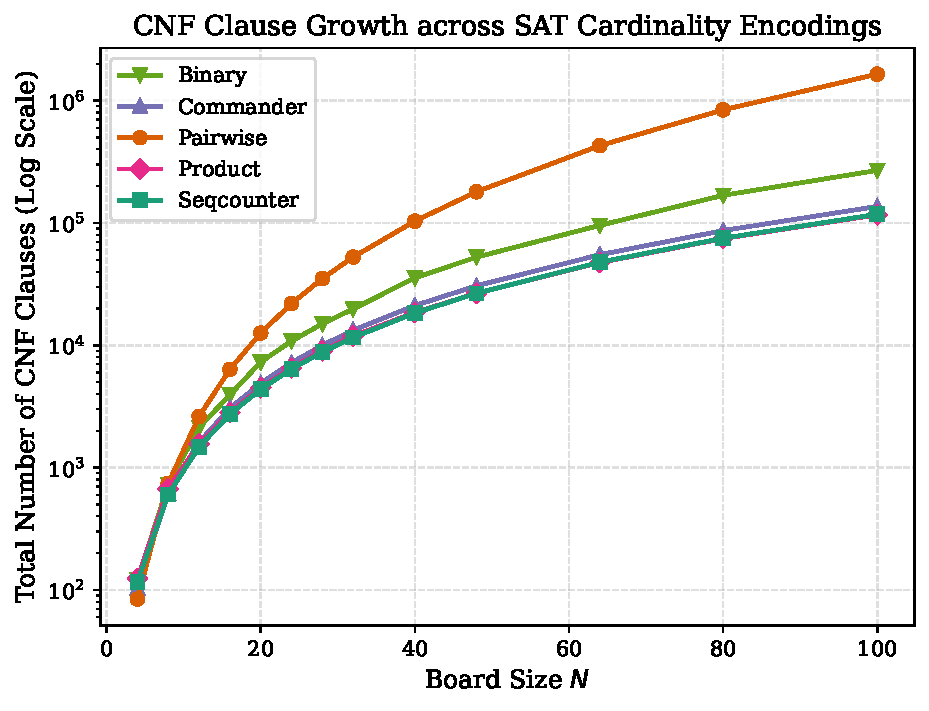
\includegraphics[width=\textwidth]{figs/fig1_clauses_vs_n.pdf}
        \caption{Clause count versus $N$ (log scale).}
        \label{fig:clauses_scaling}
    \end{subfigure}
    \hfill
    \begin{subfigure}[b]{0.48\textwidth}
        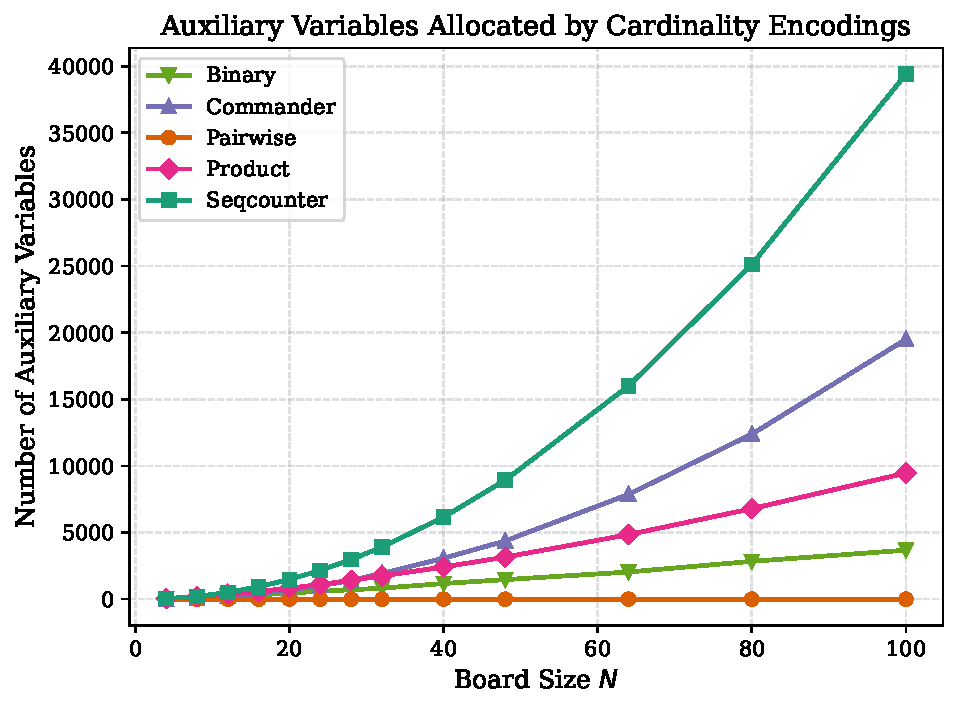
\includegraphics[width=\textwidth]{figs/fig2_aux_vars_vs_n.pdf}
        \caption{Auxiliary variables versus $N$.}
        \label{fig:aux_vars_scaling}
    \end{subfigure}
    \caption{CNF growth under the five encodings (Experiment A).}
    \label{fig:cnf_growth}
\end{figure*}

\begin{figure}[t]
    \centering
    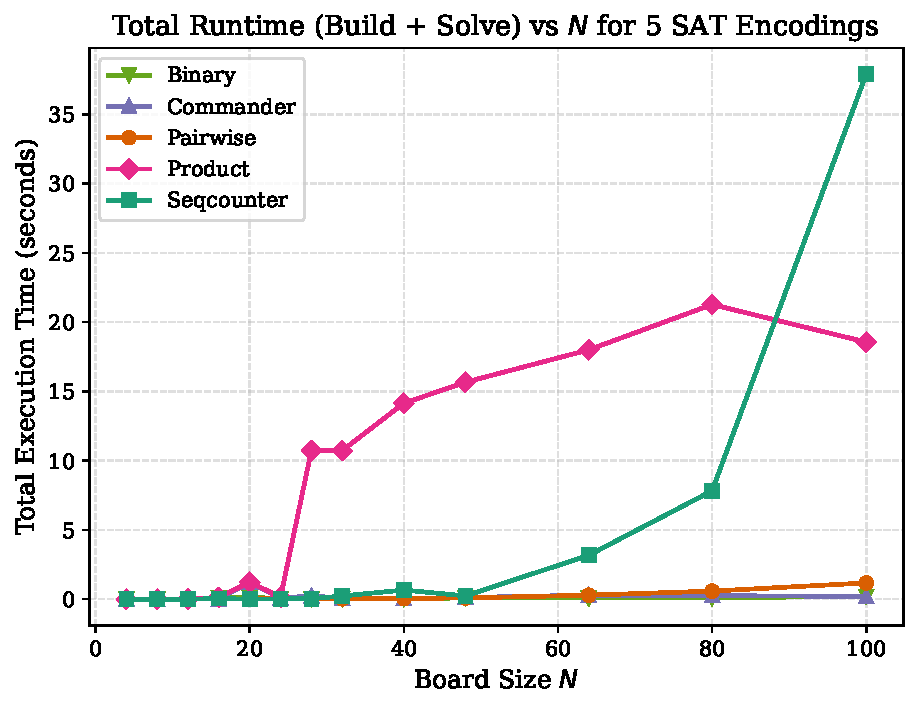
\includegraphics[width=0.72\textwidth]{figs/fig3_encoding_runtime.pdf}
    \caption{Total runtime versus $N$ on Glucose~4 (Experiment A).}
    \label{fig:encoding_runtime}
\end{figure}

Observations:
\begin{enumerate}
    \item Pairwise matches theory: $1.65\times 10^6$ clauses at $N=100$, 13.9$\times$ Sequential Counter, and the highest build cost (0.63~s).
    Search itself stays cheap (0.58~s) because pairwise is strongly propagating.
    \item Sequential Counter is the most compact in clauses but the slowest encoding on Glucose~4 at $N=100$ (40.6~s solve).
    Compactness does not automatically yield a good CDCL heuristic landscape.
    \item Commander finishes $N=100$ in 0.16~s and Binary in 0.32~s total; both remain practical encodings in this Glucose~4 study.
    \item Product stays compact but searches poorly (20.6~s at $N=100$ and $N=80$), consistent with weaker unit-propagation strength.
\end{enumerate}

\subsection{Experiment B: SAT engines}
Sequential Counter is held fixed so that engine heuristics are isolated (Figure~\ref{fig:sat_solvers}, Table~\ref{tab:sat_engines}).

\begin{table}[t]
\centering
\caption{Total time (s) on Sequential Counter CNFs (Experiment B).}
\label{tab:sat_engines}
\begin{tabular*}{\tblwidth}{@{\extracolsep{\fill}}lrrrrr@{}}
\toprule
$N$ & Glucose~4 & CaDiCaL & MiniSat & Lingeling & MergeSat \\
\midrule
16 & 0.041 & 0.010 & 0.003 & 0.004 & 0.004 \\
32 & 0.232 & 0.179 & 0.028 & 0.013 & 0.016 \\
64 & 3.347 & 0.552 & 0.067 & 0.041 & 0.085 \\
80 & 8.791 & 3.051 & 0.147 & 0.083 & 0.106 \\
100 & 41.603 & 3.062 & 0.160 & 0.265 & 0.144 \\
\bottomrule
\end{tabular*}
\end{table}

\begin{figure}[t]
    \centering
    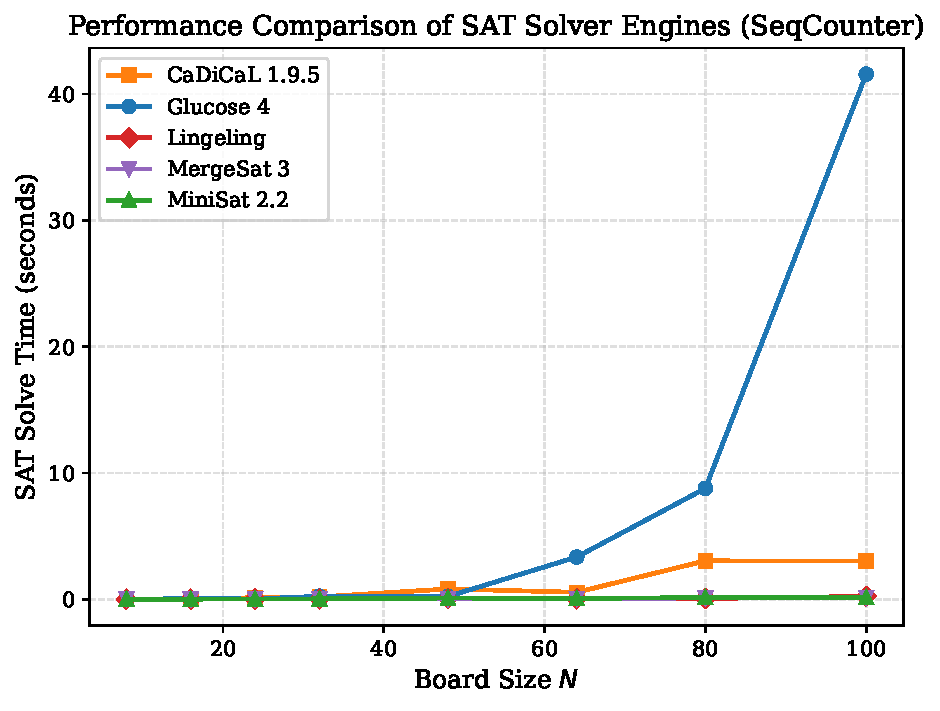
\includegraphics[width=0.72\textwidth]{figs/fig4_sat_solvers_comparison.pdf}
    \caption{SAT engine comparison on Sequential Counter (Experiment B).}
    \label{fig:sat_solvers}
\end{figure}

At $N=100$, MergeSat~3 is fastest (0.14~s), followed by MiniSat~2.2 (0.16~s), Lingeling (0.27~s), CaDiCaL (3.06~s), and Glucose~4 (41.60~s).
The same CNF is therefore not a single ``SAT runtime''; it is an interaction between encoding and restart/clause-management policy.

\subsection{Experiment C: paradigms}
Table~\ref{tab:paradigm_data} and Figure~\ref{fig:paradigm_comp} compare SAT Sequential Counter (Glucose~4) with MIP and CP.

\begin{table*}[t]
\centering
\caption{Total wall-clock time (s). ``Lic.'' denotes the CPLEX Community Edition size limit, not a timeout. Gurobi used the authenticated WLS academic license.}
\label{tab:paradigm_data}
\begin{tabular*}{\textwidth}{@{\extracolsep{\fill}}rrrrrrr@{}}
\toprule
$N$ & SAT Seq. & Gurobi & CP-SAT AD & CP-SAT 2D & CPLEX MIP & CPLEX CP \\
\midrule
8 & 0.001 & 0.013 & 0.017 & 0.014 & 0.011 & 0.029 \\
16 & 0.041 & 0.035 & 0.032 & 0.030 & 0.017 & 0.033 \\
28 & 0.033 & 0.010 & 0.064 & 0.044 & 0.033 & 0.031 \\
32 & 0.257 & 0.025 & 0.081 & 0.046 & Lic. & 0.028 \\
44 & 0.262 & 0.053 & 0.126 & 0.077 & Lic. & 0.029 \\
48 & 0.210 & 0.015 & 0.175 & 0.107 & Lic. & 0.035 \\
64 & 3.272 & 0.022 & 0.265 & 0.175 & Lic. & 0.033 \\
80 & 8.659 & 0.056 & 0.607 & 0.370 & Lic. & 0.042 \\
100 & 42.707 & 0.067 & 0.770 & 0.511 & Lic. & 0.053 \\
\bottomrule
\end{tabular*}
\end{table*}

\begin{figure}[t]
    \centering
    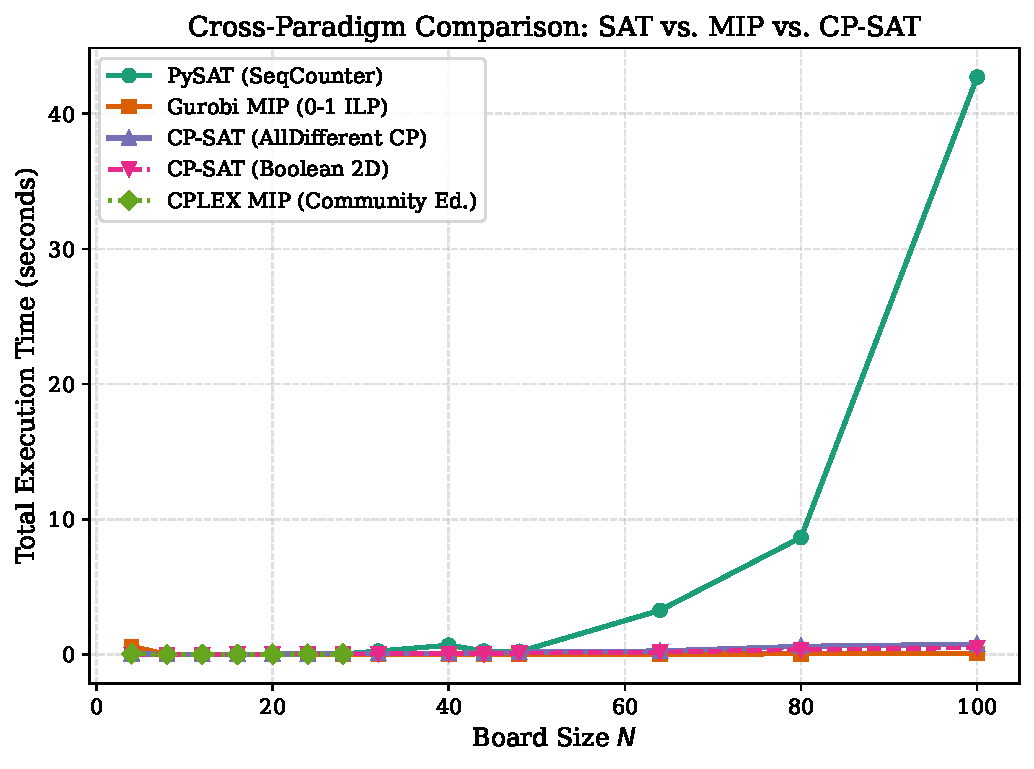
\includegraphics[width=0.75\textwidth]{figs/fig5_paradigm_comparison.pdf}
    \caption{Cross-paradigm runtimes (Experiment C). Licence-limited MIP points are omitted from the curves.}
    \label{fig:paradigm_comp}
\end{figure}

\begin{enumerate}
    \item Authenticated Gurobi WLS solves every tested board through $N=100$; the $N=100$ model has 10{,}000 binaries and takes 0.067~s total.
    \item CPLEX MIP hits the promotional 1000-variable cap at $N=32$ (\texttt{1024 vars, 186 consts, CPLEX code=1016}).
    CPLEX CP Optimizer continues and remains near 0.03~s through $N=100$ in this feasibility setting.
    \item Both CP-SAT formulations beat Glucose~4 Sequential Counter by more than an order of magnitude at $N=100$.
    The Boolean 2D model is slightly faster than AllDifferent on these mid-size boards, while AllDifferent uses far fewer variables.
\end{enumerate}

\subsection{Experiment D: scalability}
Figure~\ref{fig:scalability} and Table~\ref{tab:scale} stress $N\ge 100$ under the same 60-second request.

\begin{table}[t]
\centering
\caption{Scalability frontier (Experiment D). Times are total wall-clock seconds.}
\label{tab:scale}
\begin{tabular*}{\tblwidth}{@{\extracolsep{\fill}}lrrr@{}}
\toprule
$N$ & CP-SAT AllDiff & SAT Seq.\ (Glucose~4) & Gurobi MIP \\
\midrule
100 & 0.82 (OK) & 51.43 (OK) & 0.14 (OK) \\
150 & 10.10 (OK) & timeout$^\ast$ & 0.11 (OK) \\
200 & 14.98 (OK) & timeout$^\ast$ & 0.63 (OK) \\
300 & timeout (60.1) & timeout$^\ast$ & 0.72 (OK) \\
500 & timeout (60.1) & timeout$^\ast$ & 2.14 (OK) \\
\bottomrule
\end{tabular*}
\end{table}
{\footnotesize $^\ast$SAT interrupt is sluggish: logged totals are 94~s ($N=200$), 213~s ($N=300$), and 463~s ($N=500$), all labelled \texttt{TIMEOUT}; $N=150$ also times out at 61~s.}

\begin{figure}[t]
    \centering
    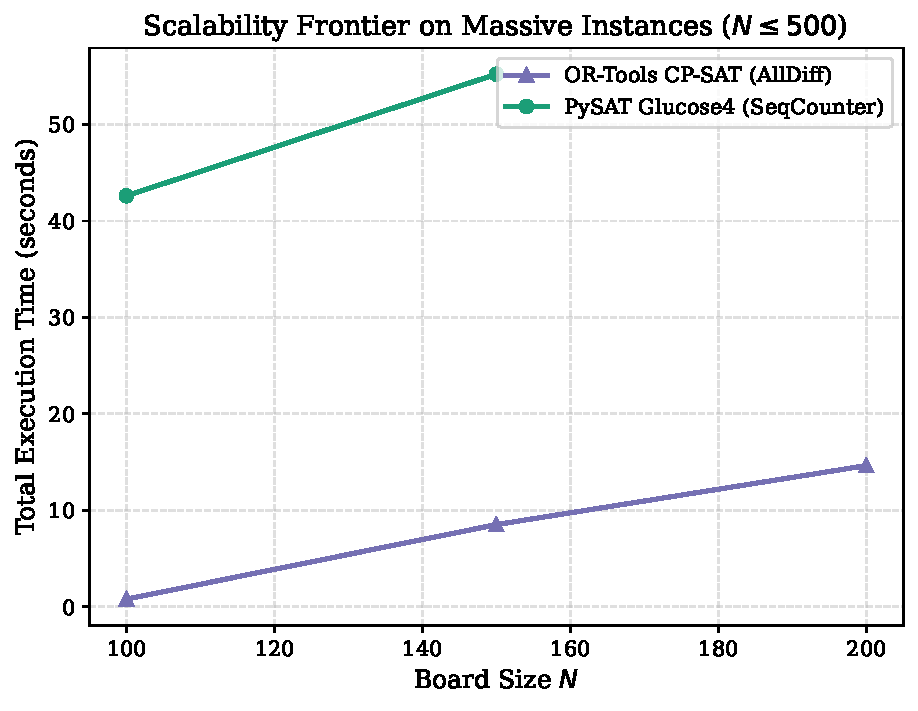
\includegraphics[width=0.72\textwidth]{figs/fig6_scalability_frontier.pdf}
    \caption{Scalability up to $N=500$ (Experiment D).}
    \label{fig:scalability}
\end{figure}

Gurobi with the authenticated WLS academic license solves every tested size through $N=500$; at the largest size the model has 250{,}000 binary variables and completes in 2.14~s total.
CP-SAT AllDifferent solves $N=200$ in 14.98~s but reaches the 60-second cap at $N=300$ and $N=500$.
SAT Sequential Counter times out from $N=150$: its $N=200$ formula has $198{,}802$ variables and $475{,}612$ clauses, while at $N=500$ it has $1{,}247{,}002$ variables and $2{,}989{,}012$ clauses.
The SAT interrupt is sluggish on large instances, so the observed wall times (94--463~s) exceed the requested 60~s limit even though each run is labelled \texttt{TIMEOUT}.

\begin{figure}[t]
    \centering
    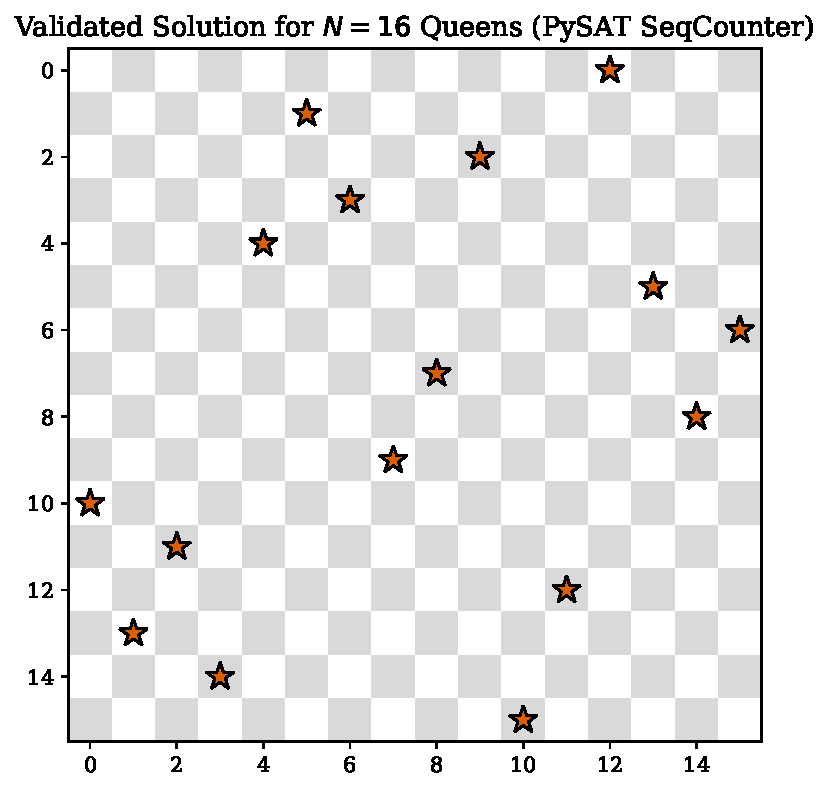
\includegraphics[width=0.55\textwidth]{figs/fig7_chessboard_n16.pdf}
    \caption{Validator-approved placement for $N=16$ produced by PySAT.}
    \label{fig:chessboard}
\end{figure}

\subsection{Experiment E: seed stability}
Five seeds at $N=32$ give Sequential Counter totals with mean $0.237$~s and sample standard deviation $0.010$~s.
Product remains slower and more variable (mean $12.210$~s, sd $0.870$~s).
Pairwise stays fast (mean $0.040$~s).
CP-SAT AllDifferent has mean $0.071$~s and sd $0.009$~s.
Ranking of methods is therefore not an artefact of a single unlucky seed.
Table~\ref{tab:stability} lists the raw totals.

\begin{table}[t]
\centering
\caption{Total time (s) over five seeds at $N=32$ (Experiment E).}
\label{tab:stability}
\begin{tabular*}{\tblwidth}{@{\extracolsep{\fill}}lrrrr@{}}
\toprule
Seed & Pairwise & Seq.\ Counter & Product & CP-SAT AD \\
\midrule
1 & 0.033 & 0.235 & 12.139 & 0.078 \\
2 & 0.039 & 0.253 & 13.725 & 0.058 \\
3 & 0.031 & 0.227 & 11.771 & 0.081 \\
4 & 0.063 & 0.236 & 11.575 & 0.071 \\
5 & 0.033 & 0.234 & 11.844 & 0.069 \\
\bottomrule
\end{tabular*}
\end{table}

\section{Discussion}
\label{sec:discussion}

\paragraph{Encoding versus engine.}
On Glucose~4, Commander/Binary beat Sequential Counter even though Sequential Counter posts fewer clauses.
On MergeSat, Lingeling, and MiniSat, the same Sequential Counter formula becomes easy.
Reporting ``SAT is slow on $N$-Queens'' without naming encoding and engine would be misleading.

\paragraph{How the authenticated Gurobi run changes the scalability result.}
The 1D model uses $N$ domain variables and matching-based pruning~\cite{regin1994filtering}.
SAT Sequential Counter at $N=200$ already allocates $198{,}802$ variables and $475{,}612$ clauses, and Glucose~4 cannot finish within 60~s.
The authenticated Gurobi academic WLS license accepted models through $N=500$ and solved the 250{,}000-binary instance in 2.14~s.
This result applies to the active licensed configuration and measured feasibility model; it should not be generalised to other academic license types or machines.

\paragraph{Feasibility, not optimisation.}
$N$-Queens has a constant objective.
MIP's usual strength---tight relaxations for a non-trivial objective---is only partly used.
The comparison is still fair as a CSP, which is the problem we actually implemented.

\paragraph{Honesty about licences.}
The refreshed run authenticated Gurobi through WLS and encountered no Gurobi size limit through $N=500$.
The CPLEX Community Edition MIP cap remains a licensing constraint, not an algorithmic proof that MIP fails.
The logs keep vendor error strings so that reviewers can audit the CPLEX limit.

\section{Threats to validity}
\label{sec:threats}

\begin{itemize}
    \item \textbf{Single machine, single timeout.} Rankings may change on a server-class CPU, with more threads, or with a one-hour cutoff (Experiment D would likely move).
    \item \textbf{Licence envelope.} The Gurobi results depend on the authenticated WLS academic license available during this run; another academic license type may impose a model-size cap. CPLEX MIP remains subject to its Community Edition cap.
    \item \textbf{SAT interrupt.} PySAT/Glucose did not always stop at 60~s on huge formulas; TIMEOUT is still the correct scientific label, but wall-clock is larger than the requested budget.
    \item \textbf{No symmetry breaking} (lex-leader / orbit restrictions). Adding it could change SAT/CP gaps.
    \item \textbf{Existence only.} We do not count all solutions or solve $N$-Queens completion~\cite{gent2017nqueens}.
\end{itemize}

\section{Data Availability}
\label{sec:data}

As required for B{\`a}o c{\'a}o BTL s{\^o}~1, the repository that stores the source code and the experimental results of this assignment is public:

\begin{center}
\textbf{\url{https://github.com/YwliF/BTL_01}}
\end{center}

\noindent The Git remote of the working copy is \texttt{https://github.com/YwliF/BTL\_01.git}.
Concrete paths inside that repository:
\begin{itemize}
    \item source: \texttt{src/nqueens/};
    \item tests: \texttt{tests/} and \texttt{scripts/run\_correctness\_tests.py};
    \item Experiments A--E: \texttt{results/raw/exp\_a\_encodings.csv}, \texttt{exp\_b\_sat\_solvers.csv}, \texttt{exp\_c\_paradigms.csv}, \texttt{exp\_d\_scalability.csv}, \texttt{exp\_e\_stability.csv};
    \item figures: \texttt{results/figures/} and \texttt{paper/figs/};
    \item this report: \texttt{paper/main.tex}.
\end{itemize}
Reproduction: install \texttt{requirements.txt}, optionally configure Gurobi WLS via environment variables (credentials are never committed), run \texttt{python scripts/run\_benchmarks.py --mode full}, then \texttt{python scripts/generate\_plots.py}, then compile this manuscript with \texttt{python scripts/compile\_paper.py}.

\section{Conclusion}
\label{sec:conclusion}

This BTL~1 report implemented exact $N$-Queens solving across SAT, MIP, and CP, compared five cardinality encodings and five CDCL engines, and published the measurements.
On the recorded data, Commander and Binary encodings are the robust SAT choices for Glucose~4; MergeSat~3, MiniSat~2.2, and Lingeling dominate Glucose~4 on Sequential Counter; authenticated Gurobi solves through $N=500$ in 2.14~s, while CP-SAT solves through $N=200$ and times out at $N=300$ and $N=500$; CPLEX MIP remains limited by its Community Edition cap.
All code and CSV results are available at \url{https://github.com/YwliF/BTL_01}.

Future work includes symmetry breaking, a SAT portfolio that pairs Sequential Counter with MergeSat rather than Glucose~4, and repeating the MIP comparison across additional license configurations and hardware.

\printcredits

\bibliographystyle{cas-model2-names}
\bibliography{references}

\end{document}
